\documentclass{ctexbeamer}

  \mode<presentation>
  {
    \usetheme{CambridgeUS}      % or try Darmstadt, Madrid, Warsaw, ...
    \usecolortheme{default} % or try albatross, beaver, crane, ...
    \usefonttheme{default}  % or try serif, structurebold, ...
    \setbeamertemplate{navigation symbols}{}
    \setbeamertemplate{caption}[numbered]
  } 
  
  \usepackage[english]{babel}
  \usepackage[utf8x]{inputenc}
  
  \title[NIPS2017]{Associative Embedding: End-to-End Learning for Joint Detection and Grouping Alejandro}
  
  \author{报告人:陈伟航\\}
  
  \institute{\bf South China University of Technology}
  %\textsc {Industrial Training Presentation }
  
  \date{$31^{\text{th}}$ May 2018}
  
  \begin{document}
  
  \begin{frame}
    \titlepage
  \end{frame}
  
  
  \section{Introduction : Online Tax Payment}
  
  \begin{frame}{Online Tax Payment(OLTAS)}
  
  \begin{itemize}
    \item OLTAS is a private owned product used by Yes Bank.
    \item A system which can integrate with internet portal and provide facility of making tax payments to their end internet portal users.
  \end{itemize}
  
  % Commands to include a figure:
  \begin{figure}
  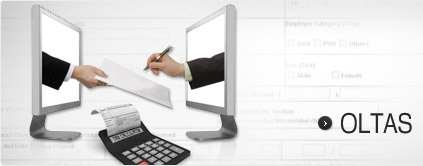
\includegraphics[width=5cm ,height= 3cm]{fig/oltas-header.jpg}
  \caption{\label{fig:your-figure-1}OLTAS}
  \end{figure}
  \vskip 1cm
  
  \end{frame}
  %%%%%%%%%%%%%%%
  
  \section{MySpace and OLTAS}
  
  \begin{frame}{MySpace}
  
  \begin{itemize}
    \item OLTAS is a part of MySpace.
    \item MySpace is totally for customer’s space, where different types of services like insurance schemes , cheque printing, online payments, gifts and voucher offers provided by Yes Bank under one application.
  
  \end{itemize}
  
  % Commands to include a figure:
  \begin{figure}
  
\includegraphics[width=5cm ,height= 3cm]{fig/multitasking_cartoon.jpg}
  \caption{\label{fig:your-figure}MySpace}
  \end{figure}
  \vskip 1cm
  
  \end{frame}
  
  %%%%%%%%%%%%%%%
  
  \section{How it Works}
  
  \begin{frame}{Yes Bank and NSDL}
  
  \begin{itemize}
    \item Yes Bank is a depository participant of NSDL.
  
    \item Yes Bank act as a middle man in the process of online tax payment.
  
  \end{itemize}
  
  \vskip 1cm
  \end{frame}
  
  \begin{frame}{NSDL}
  
  \begin{itemize}
    \item NSDL is promoted byIndustrial Development Bank of India Limited(IDBI) - the largest development bank of India.
  \item NSDLis an Indian central securities depository.
  
  \end{itemize}
  \vskip 1cm
  
  \end{frame}
  
  
  %%%%%%%%%%%%%%%%
  
  \section{Benefits}
  
  \begin{frame}{Benefits}
  
  \begin{block}{From customer’s point of view}
  \end{block}
  \begin{itemize}
  
  %\end{}{itemize}
  \item Ease of access : Tax payers can track online the status of their challans deposited in banks
  \item Secure
    \item Check present status of challan
    \item Get Confirmation
  
  \end{itemize}
  
  \begin{block}{From Bank’s point of view}
  \end{block}
  \begin{itemize}
  
  %\end{}{itemize}
  \item Provide multiple services
  \item Make Business
  \item Increase Brand Value
  \end{itemize}
  
  \vskip 1cm
  \end{frame}
  
  %---------------------
  \section{References}
  \begin{frame}
  \frametitle{References}
  \begin{itemize}
  \item \url{https://nsdl.co.in/about/why.php/}
  \item \url{http://deic.uab.es/~iblanes/beamer_gallery/} \\
  \item \url{http://www.idbi.com/online-tax-payment.asp} \\
  \end{itemize}
  
  
  \begin{block}{E-Books}
  \begin{itemize}
  
  %\end{}{itemize}
  \item Programming ASP.NET 3.5 
  \item The Indian Financial System: Markets, Institutions and Services
  \end{itemize}
  \end{block}
  \vskip 1cm
  \end{frame}
  
  
  \section{End of Presentation}
  \begin{frame}
  \begin{itemize}[<+-| alert@+>]
  \item Thank You.
  \end{itemize}
  \end{frame}
  
  \end{document}
  